%%%%%%%%%%%%%%%%%%%%%%%%%%%%%%%%%%%%%%%%%%%%%%%%%%%
%% P3: Phenomenology of Particle Physics                         
%%
%% Author:  André Rubbia                   		 
%%
%% Figure 20.5 Measured invariant mass of the muon pair in proton--nucleus interactions.
%%
%% This work is licensed under the Creative Commons Attribution 4.0 International License. 
%% To view a copy of this license, visit http://creativecommons.org/licenses/by/4.0/ or 
%% send a letter to Creative Commons, PO Box 1866, Mountain View, CA 94042, USA.
%%
%%%%%%%%%%%%%%%%%%%%%%%%%%%%%%%%%%%%%%%%%%%%%%%%%%%

\documentclass[a4paper,10pt]{article}

\usepackage[T1]{fontenc}
\usepackage[utf8]{inputenc}
\usepackage{lmodern}
\usepackage[labelfont=bf]{caption}
\usepackage{upgreek}

\usepackage{tikz}
\usepackage{pgfplots}
\pgfplotsset{compat=1.17}
\usepgfplotslibrary{ternary}
\usepgfplotslibrary{fillbetween}
\usepgfplotslibrary{external}

\def\d{\mathrm{d}}

\begin{document}

%%%%%%%%%%%%%%%%   FIGURE  %%%%%%%%%%%%%%%%%%%%%%%%%%%%%%
\begin{figure}[tb]
\centering
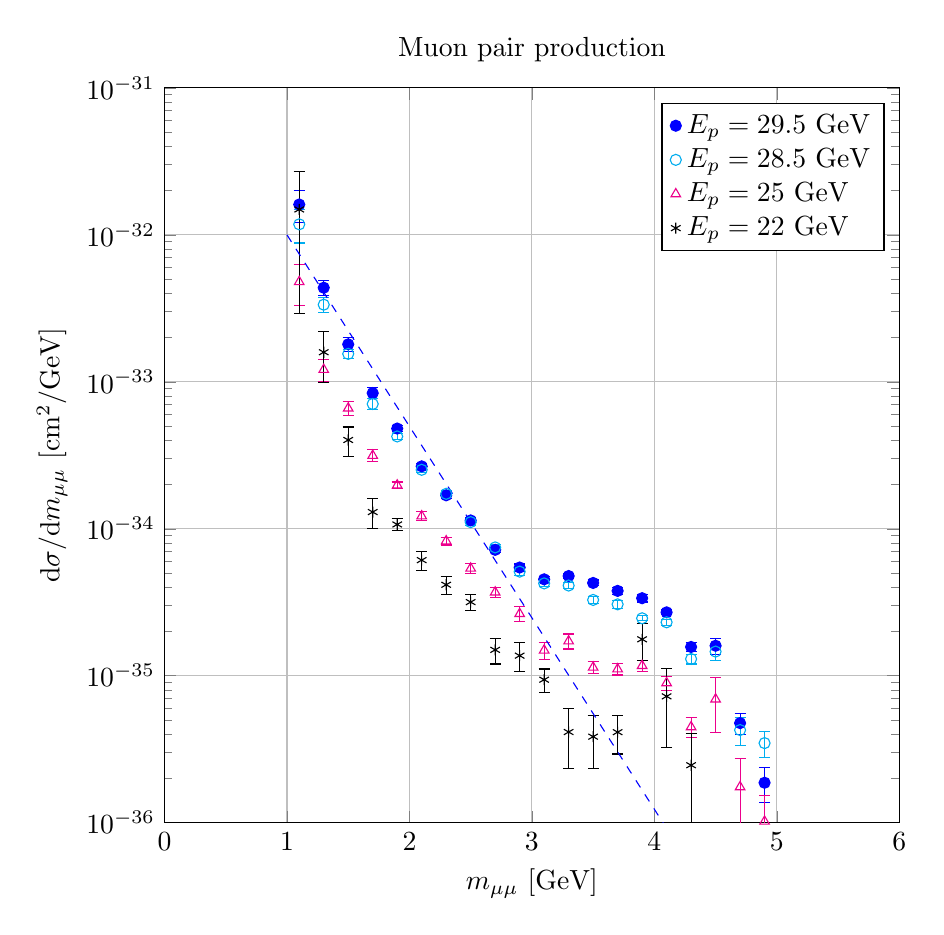
\begin{tikzpicture}[scale=1.]
    \begin{semilogyaxis}[
    width=0.9\textwidth,
    height=0.9\textwidth,
        title=Muon pair production,
        xlabel={$m_{\mu\mu}$ [GeV]},
        ylabel={$\d\sigma/\d m_{\mu\mu}$ [cm$^2$/GeV]},
        xmin=0, xmax=6,
        ymin = 1e-36, ymax=1e-31,
        minor y tick num=1,
        grid = major,
	legend cell align = {left},
	legend entries={
	$E_p=29.5$~GeV,
	$E_p=28.5$~GeV,
	$E_p=25$~GeV,
	$E_p=22$~GeV
        },
    ]

%%% Ep=29.5 GeV
    \addplot[
    color=blue,
    only marks, mark=*,
    error bars/.cd,
    y dir=both, y explicit
    ]
    coordinates {
(1.1,1.61e-32)+-(0,0.4e-32)
(1.3,4.37e-33)+-(0,0.5e-33)
(1.5,1.80e-33)+-(0, 0.2e-33)
(1.7,8.38e-34)+-(0, 0.7e-34)
(1.9,4.81e-34)+-(0, 0.2e-34)
%%
(2.1,2.66e-34)+-(0,0.1e-34)
(2.3,1.69e-34)+-(0,0.08e-34)
(2.5,1.14e-34)+-(0,0.05e-34)
(2.7,7.19e-35)+-(0,0.3e-35)
(2.9,5.45e-35)+-(0,0.3e-35)
%%
(3.1,4.53e-35)+-(0, 0.2e-35)
(3.3,4.77e-35)+-(0, 0.2e-35)
(3.5,4.28e-35)+-(0, 0.2e-35)
(3.7,3.78e-35)+-(0, 0.2e-35)
(3.9,3.37e-35)+-(0, 0.2e-35)
%%
(4.1,2.70e-35)+-(0, 0.1e-35)
(4.3,1.57e-35)+-(0, 0.1e-35)
(4.5,1.60e-35)+-(0, 0.2e-35)
(4.7,4.76e-36)+-(0, 0.8e-36)
(4.9,1.87e-36)+-(0, 0.5e-36)
};

%%% Ep=28.5 GeV
    \addplot[
    color=cyan,
    only marks,mark=o,
    error bars/.cd,
    y dir=both, y explicit
    ]
    coordinates {
(1.1,1.18e-32 )+-(0,  0.3e-32)
(1.3,3.35e-33 )+-(0,  0.4e-33)
(1.5,1.55e-33 )+-(0,  0.1e-33)
(1.7,7.07e-34 )+-(0,  0.6e-34)
(1.9,4.25e-34 )+-(0,  0.2e-34)
%
(2.1,2.52e-34 )+-(0,  0.1e-34)
(2.3,1.73e-34 )+-(0,  0.08e-34)
(2.5,1.11e-34 )+-(0,  0.06e-34)
(2.7,7.47e-35 )+-(0,  0.3e-35)
(2.9,5.11e-35 )+-(0,  0.3e-35)
%
(3.1,4.25e-35 )+-(0,  0.2e-35)
(3.3,4.11e-35 )+-(0,  0.2e-35)
(3.5,3.28e-35 )+-(0,  0.2e-35)
(3.7,3.06e-35 )+-(0,  0.2e-35)
(3.9,2.46e-35 )+-(0,  0.1e-35)
%
(4.1,2.31e-35 )+-(0,  0.1e-35)
(4.3,1.30e-35 )+-(0,  0.1e-35)
(4.5,1.46e-35 )+-(0,  0.2e-35)
(4.7,4.27e-36 )+-(0,  0.9e-36)
(4.9,3.48e-36 )+-(0,  0.7e-36)
};

%%% Ep=25 GeV
    \addplot[
    color=magenta,
    only marks,mark=triangle,
    error bars/.cd,
    y dir=both, y explicit
    ]
    coordinates {
(1.1,0.479e-32 )+-(0,  0.15e-32)
(1.3,1.21e-33 )+-(0,  0.2e-33)
(1.5,0.661e-33 )+-(0,  0.07e-33)
(1.7,3.15e-34 )+-(0,  0.3e-34)
(1.9,1.98e-34 )+-(0,  0.1e-34)
%
(2.1,1.22e-34 )+-(0,  0.09e-34)
(2.3,0.825e-34 )+-(0,  0.05e-34)
(2.5,0.538e-34 )+-(0,  0.04e-34)
(2.7,3.70e-35 )+-(0,  0.3e-35)
(2.9,2.64e-35 )+-(0,  0.3e-35)
%
(3.1,1.49e-35 )+-(0,  0.2e-35)
(3.3,1.72e-35 )+-(0,  0.2e-35)
(3.5,1.14e-35 )+-(0,  0.1e-35)
(3.7,1.11e-35 )+-(0,  0.1e-35)
(3.9,1.17e-35 )+-(0,  0.1e-35)
%
(4.1,0.893e-35 )+-(0,  0.1e-35)
(4.3,0.448e-35 )+-(0,  0.07e-35)
(4.5,0.692e-35 )+-(0,  0.28e-35)
(4.7,1.75e-36 )+-(0,  1.0e-36)
(4.9,1.02e-36 )+-(0,  0.5e-36)
};

%%% Ep=22 GeV
    \addplot[
    color=black,
    only marks,mark=asterisk,
    error bars/.cd,
    y dir=both, y explicit
    ]
    coordinates {
(1.1,1.49e-32 )+-(0,  1.2e-32)
(1.3,1.59e-33 )+-(0,  0.6e-33)
(1.5,0.402e-33 )+-(0,  0.09e-33)
(1.7,1.30e-34 )+-(0,  0.3e-34)
(1.9,1.07e-34 )+-(0,  0.1e-34)
%
(2.1,0.612e-34 )+-(0,  0.09e-34)
(2.3,0.416e-34 )+-(0,  0.06e-34)
(2.5,0.317e-34 )+-(0,  0.04e-34)
(2.7,1.50e-35 )+-(0,  0.3e-35)
(2.9,1.37e-35 )+-(0,  0.3e-35)
%
(3.1,0.940e-35 )+-(0,  0.17e-35)
(3.3,0.414e-35 )+-(0,  0.18e-35)
(3.5,0.385e-35 )+-(0,  0.15e-35)
(3.7,0.413e-35 )+-(0,  0.12e-35)
(3.9,1.77e-35 )+-(0,  0.5e-35)
%
(4.1,0.724e-35 )+-(0,  0.4e-35)
(4.3,0.246e-35 )+-(0,  0.16e-35)
};

    \addplot [blue,thin,dashed,domain=1:5] {1e-32*exp(-3*(x-1))};

   \end{semilogyaxis}
\end{tikzpicture}%
\caption{Measured invariant mass of the muon pair in proton--nucleus interactions for
incident proton energies of 22, 25, 28.5, and 29.5~GeV. Data taken with permission from
J.~H. Christenson, G.~S. Hicks, L.~M. Lederman, P.~J. Limon, B.~G. Pope, and
  E.~Zavattini, ``{Observation of muon pairs in high-energy hadron
  collisions},'' {\em Phys. Rev.}, vol.~D8, pp.~2016--2034, 1972.
The dashed line illustrates an exponentially decaying spectrum.}
\end{figure}
%
%%%%%%%%%%%%%%%%   END FIGURE  %%%%%%%%%%%%%%%%%%%%%%%%%%%%%%
%
\end{document}
